Este capítulo describe el diseño e implementación de Voctomix~2.0: la arquitectura del
sistema, sus componentes principales y las decisiones técnicas adoptadas durante el
desarrollo. Para cada módulo se exponen los retos encontrados y los mecanismos
implementados para resolverlos.

El trabajo comenzó con una fase de exploración sobre Voctomix~1.0 para familiarizarse
con la herramienta antes de abordar la versión más reciente. Durante esas primeras
semanas se estudió en detalle el fichero de configuración \texttt{default.ini}, se
comprendió el funcionamiento del protocolo de puertos TCP de entrada de las cámaras
(10000, 10001, 10002), se analizaron los flujos de previsualización de la interfaz gráfica y se exploró el funcionamiento de los composites.
Esta inmersión en la versión anterior resultó clave para entender los fundamentos del
pipeline GStreamer, la comunicación cliente-servidor, y la
arquitectura del sistema, y sirvió de base sólida para dar el salto a Voctomix~2.0.

La figura~\ref{fig:diagrama_sistema} ofrece una visión global del sistema completo:
las fuentes de señal, el núcleo de procesamiento, las salidas, la interfaz de control, la capa de telemetría, etc. Este diagrama sirve de hilo conductor para los apartados que
siguen, cada uno de los cuales profundiza en uno de sus bloques.

\begin{figure}[H]
  \centering
  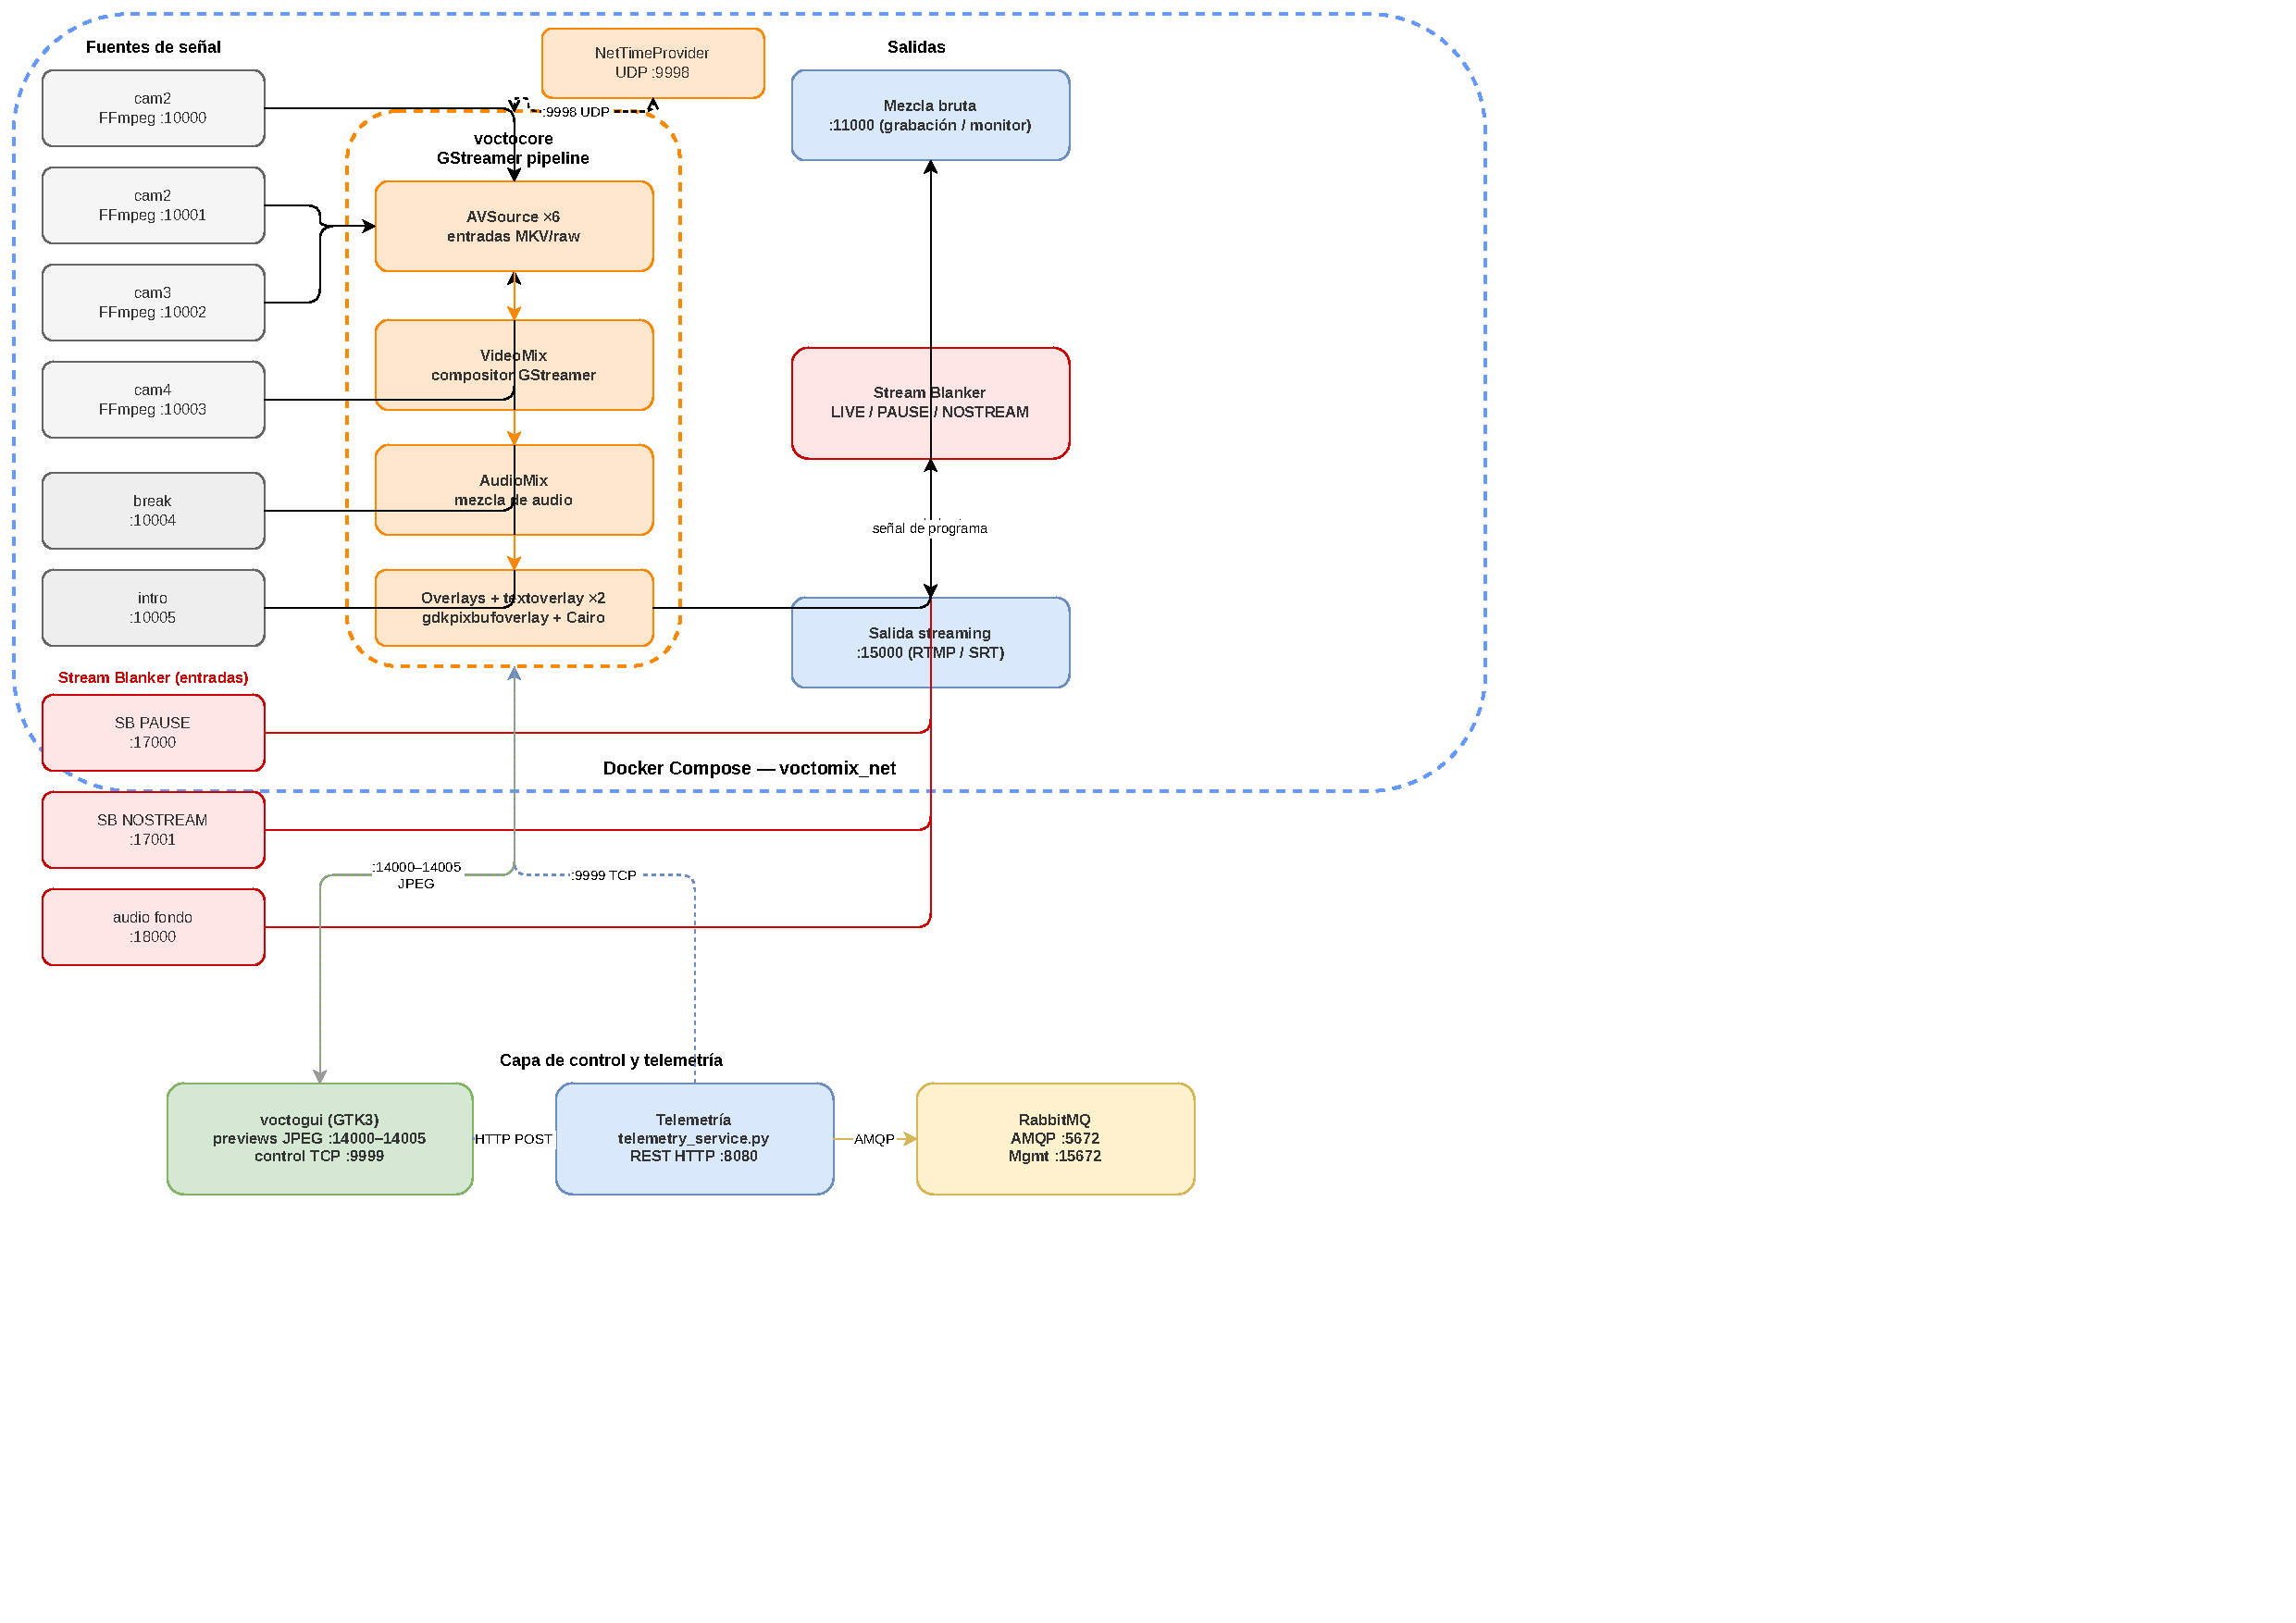
\includegraphics[width=\textwidth]{figuras/diagrama_sistema}
  \caption{Arquitectura global del sistema Voctomix~2.0.}
  \label{fig:diagrama_sistema}
\end{figure}

La tabla~\ref{tab:puertos_sistema} recoge los puertos TCP/UDP del sistema y su función.

\begin{table}[H]
  \centering
  \caption{Puertos del sistema Voctomix 2.0.}
  \label{tab:puertos_sistema}
  \begin{tabular}{|c|l|l|}
    \hline
    \textbf{Puerto} & \textbf{Protocolo} & \textbf{Función} \\
    \hline
    9998     & UDP  & Sincronización de reloj de red GStreamer \\
    9999     & TCP  & Protocolo de control (GUI, scripts, telemetría) \\
    10000    & TCP  & Entrada cámara 1 (MKV/raw) \\
    10001    & TCP  & Entrada cámara 2 (MKV/raw) \\
    10002    & TCP  & Entrada cámara 3 (MKV/raw) \\
    10003    & TCP  & Entrada cámara 4 (MKV/raw) \\
    10004    & TCP  & Entrada fuente break (vídeo de pausa) \\
    10005    & TCP  & Entrada fuente intro (vídeo introductorio) \\
    11000    & TCP  & Salida mezcla principal en bruto \\
    12000    & TCP  & Salida principal de previsualización (GUI) \\
    14000--14005 & TCP & Salidas de previsualización comprimidas (GUI) \\
    15000    & TCP  & Salida de streaming \\
    17000    & TCP  & Entrada vídeo stream blanker PAUSE \\
    17001    & TCP  & Entrada vídeo stream blanker NOSTREAM \\
    18000    & TCP  & Entrada audio (música de fondo) \\
    8080     & HTTP & API REST del servicio de telemetría \\
    \hline
  \end{tabular}
\end{table}

% ─────────────────────────────────────────────────────────────────────────────
\section{Arquitectura del sistema}
\label{sec:arquitectura}
% ─────────────────────────────────────────────────────────────────────────────

\subsection{voctocore: núcleo multimedia}
\label{sec:voctocore}

\texttt{voctocore} es el servidor central del sistema: gestiona todo el procesamiento
multimedia, acepta las fuentes de vídeo entrantes, realiza la composición y expone los
resultados en distintos puertos TCP. Se inicializa mediante \texttt{voctocore/voctocore.py},
que instancia en orden el \texttt{Pipeline} central (grafo GStreamer), el
\texttt{ControlServer} TCP y el proveedor de tiempo de red GStreamer
(\texttt{NetTimeProvider}, puerto UDP 9998). El \texttt{Pipeline} construye
dinámicamente la cadena GStreamer a partir de la configuración INI: crea una instancia
de \texttt{AVSource} por cada fuente declarada, instancia el \texttt{VideoMix} y el
\texttt{AudioMix}, conecta el \texttt{StreamBlanker} y abre los puertos de salida.

El \texttt{ControlServer} expone el \textbf{protocolo de control} en el puerto TCP~9999:
comandos de texto plano del tipo \texttt{set\_video\_a~cam2} o
\texttt{set\_composite\_mode~pip}. Cada cambio de estado se difunde por
\textit{broadcast} a todos los clientes conectados, de forma que la interfaz gráfica,
los scripts de automatización y el servicio de telemetría mantienen una vista coherente
del sistema en todo momento.

\subsection{voctogui: interfaz gráfica de control}
\label{sec:voctogui}

\texttt{voctogui} es el cliente de control: implementado en PyGTK3, proporciona al
realizador la interfaz visual para operar el sistema en tiempo real. Se conecta al
núcleo mediante un socket TCP no bloqueante gestionado con \texttt{GObject.io\_add\_watch},
de forma que los eventos de red no bloquean el hilo principal de GTK. La GUI recibe
los flujos de previsualización de cada fuente en formato JPEG comprimido (puertos
14000--14005) para minimizar el consumo de ancho de banda, mientras que el monitor
principal recibe la mezcla final en bruto (puerto 11000).

\begin{figure}[H]
  \centering
  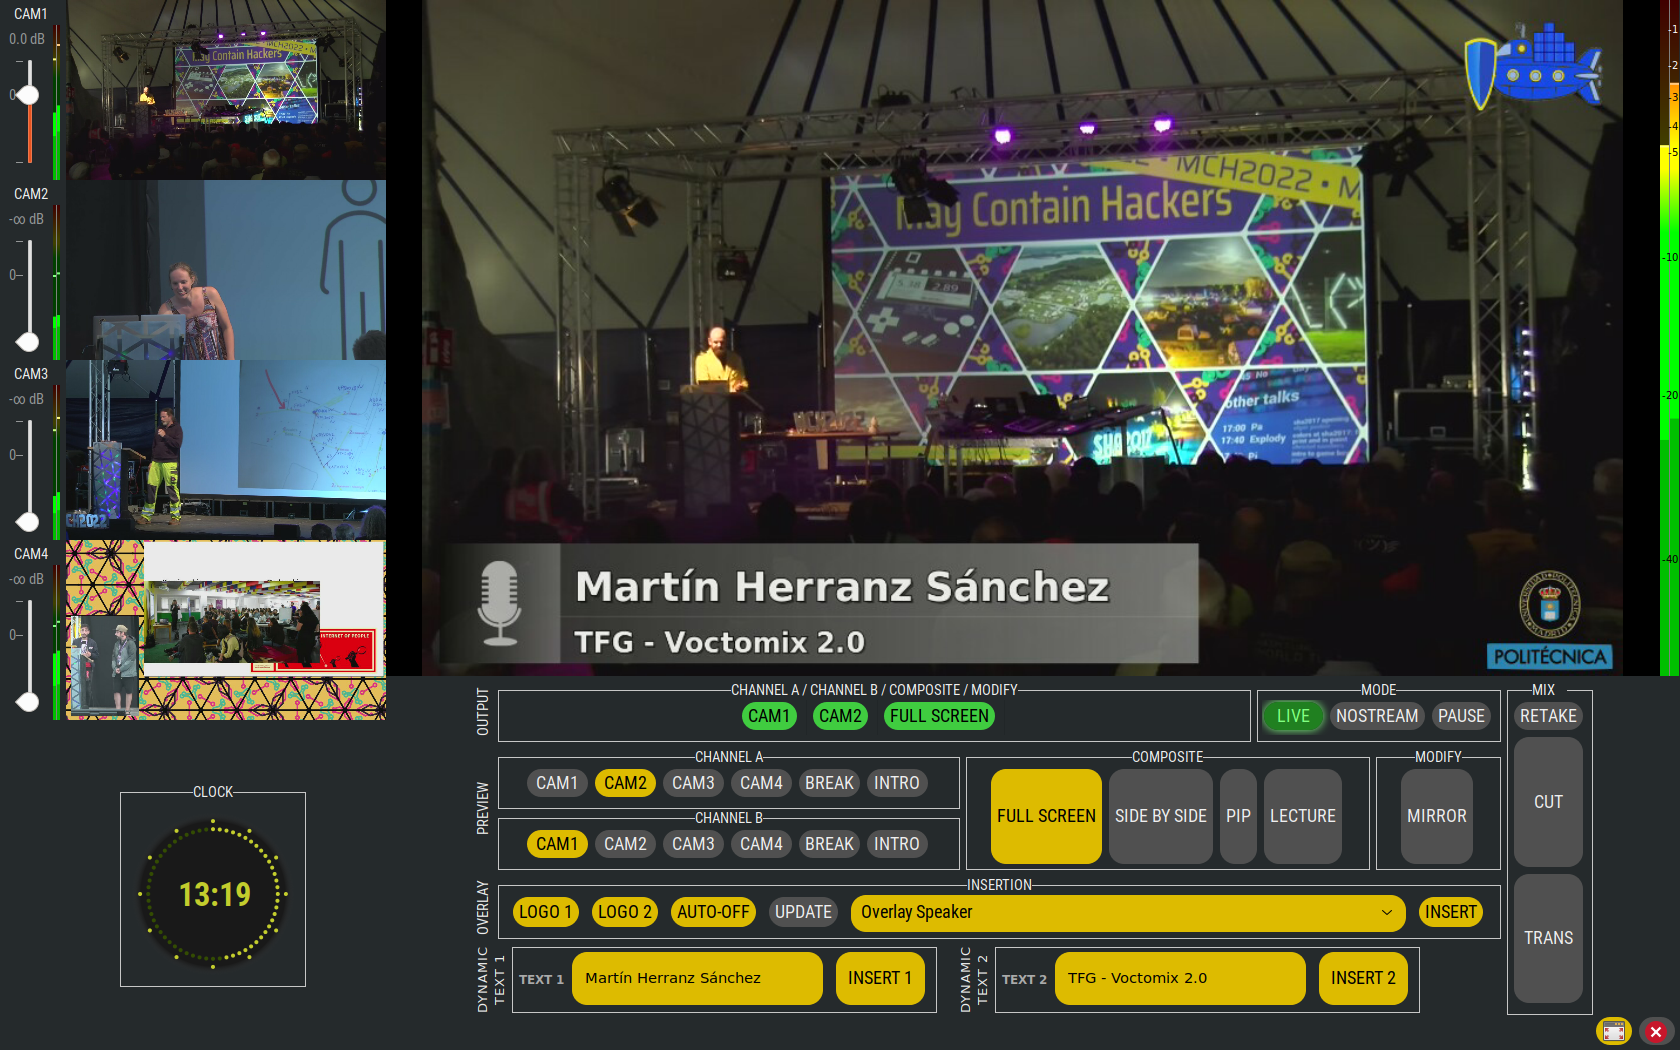
\includegraphics[width=\textwidth]{figuras/gui_completa.png}
  \caption{Interfaz gráfica completa de Voctomix~2.0 (voctogui).}
  \label{fig:gui_completa}
\end{figure}
